% !TEX root=../thesis.tex

\chapter{Background}
\label{chapter:background}
In this chapter we put the stakeholders and their needs mentioned in \Ref{sec:intro_stakeholders}
\nameref{sec:intro_stakeholders} in context of the railway system. 

The chapter begins with a description of how the railway traffic in Norway
are structured and how the infrastructure is organized. We will then describe
the stakeholders in in context of the infrastructure organization. The third
part describes different data sets and their origin. The firth part describes
how to process the data according to the stakeholders. The second to last part
presents the case study performed as part of the research method presented in
\Vref{sec:project_research}. The last part presents a framework definition of
the case study.


% !TEX root=../../thesis.tex

\section{Railway operations} % (fold)
\label{sec:railway_operations}
Major train networks are complex systems with many dynamic effects. The 
Norwegian railroad consists of 4320 km of lines \cite[p. 4]{jernbaneverketStatistikk}, transporting 60 million passenger journeys and 27 
million tons of cargo in 2012\cite[p. 9]{jernbaneverketStatistikk}. For a rail 
undertaking, there is a constant balance to be struck between capacity, demand, 
and safe and punctual operations. Safety has the highest priority between 
these concerns, and as such this thesis will focus more on capacity and 
punctual operations.\\

Punctuality is usually divided into two central metrics, punctuality and 
regularity. In the Norwegian railroad, a train is considered punctual or on 
schedule if it operates at planned points in the infrastructure within a 
margin of 3 minutes and 59 seconds, for long distance and cargo trains the 
margin is 5 minutes and 59 seconds. Punctuality (in \%) is the proportion of 
trains that arrives at their final destination within this margin.

Jernbaneverket (see \Vref{sub:subsection_jernbaneverket}) defines regularity (
in \%) as the proportion of trains operated over the number planned in the 
schedule. 

Other derived metrics include uptime, in regards to punctuality, is defined by 
Jernbaneverket from 
the hours of delay\footnote{Hours of delay due to infrastructure excluded 
traffic	management and external conditions} caused by infrastructure relative 
to sum of planned train hours\footnote{Planned train hours (passenger and 
freight trains)} per year.\cite{jernbaneverketPunklighetsTall}
\begin{equation} \label{eq:uptime}
		Uptime =
		\frac
				{
					\text{Train hours - Hours of delay}
				}
				{
					\text{Train hours}
				}\times 100 
\end{equation}\\

The operations of the railway system are divided into infrastructure owner and 
rail undertakings that provide transport on the infrastructure. In Norway the 
infrastructure is constructed, operated and maintained by the state owned 
agency Jernbaneverket. The major undertakings operating in Norway  include 
Norges Statsbaner (NSB), NSB Gjøvikbanen, CargoNet, CargoLink, and Flytoget \cite{ wiki:NorwegianRailway}. The undertakings provide exclusively either passenger 
or freight traffic.\\

Due to the size and responsibility of these organizations, there is a need for 
a division of labor and responsibility. This differs between the 
infrastructure owner and the undertakings due to their different business 
areas. Example of their individual organization charts is shown in \Ref{fig:jbv_undertaking_org_map} (undertaking) and \Ref{fig:jbv_infrastructure_org_map} (infrastructure owner).

\begin{figure}[!htbp]
	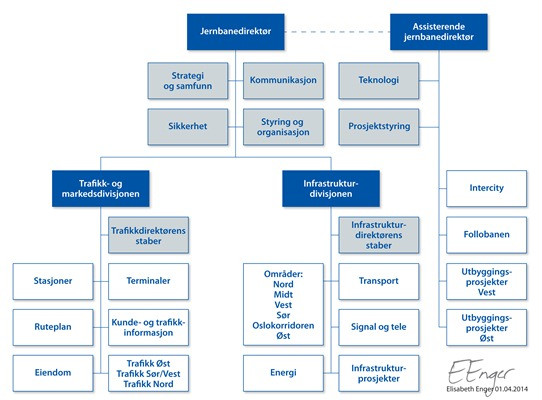
\includegraphics[width=\textwidth,center]{JBV_orgkart.jpg}
	\caption[Jernbaneverket undertaking organization]{Jernbaneverket undertaking organization \cite{sintefPresis}}
	\label{fig:jbv_undertaking_org_map}
\end{figure}

\begin{figure}[!htbp]
	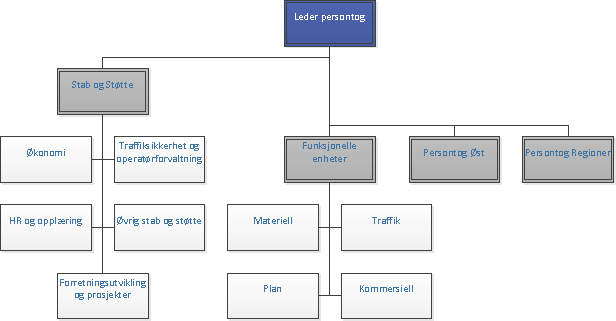
\includegraphics[width=\textwidth,center]{jbv_persontog_orgkart.png}
	\caption[Jernbaneverket infrastructure organization]{Jernbaneverket infrastructure organization \cite{jernbaneverketOrganisasjon}}
	\label{fig:jbv_infrastructure_org_map}
\end{figure}

Since most of the railway structure in Norway is single line, most crossings
have to be executed at places where sidetracks have been built, mostly this is
at stations. This means that even though one train may be experiencing delay, 
this delay may be part of a sequence of problems that can be tracked back to a 
seemingly unrelated part of the the network and a perhaps a bad decision there 
\cite{cule2011mining}.
\\

As Landex\cite{landex2009gis} says, there exist few GIS-approaches concerning
visualization of railroad capacity. Both the visualizations shown by Landex and
in \Ref{sect:backgroundExamples} \nameref{sect:backgroundExamples}, 
only seems to take into consideration whether
the trains are delayed, and the amount of delay. \\

% section railway_operations (end)

% !TEX root=../../thesis.tex

\section{Stakeholders} % (fold)
\label{sec:back_stakeholders}
When looking at the Norwegian railway, there exists several types of users which
may be taken into consideration. On the Norwegian railway operates several
companies, who all have several positions in their organization hierarchy. Each
of these positions have different responsibilities and therefor different
interests in the system. A example of such a hierarchy is presented in
\Ref{table:user_roles}.

\begin{table}[!h]\small
	\begin{tabularx}{\textwidth}{|l|X|}
		\hline
		User type & Responsibility \\
		\hline
		Railway director & Organization director\\
		\hline
		Infrastructure director & Responsibility to facilitate that the railway traffic in Norway is safe and reliable\\
		\hline
		Area director & Responsibility to coordinate traffic within a area\\
		\hline
		Stretch director & Responsibility to coordinate traffic within certain
		stretches\\
		\hline
		Segment director & Responsibility to coordinate traffic within a segment\\
		\hline
	\end{tabularx}
\caption{User roles in the Norwegian railway network}
\label{table:user_roles}
\end{table}

The hierarchy presents only relevant users from Jernbaneverket (see
\Vref{sub:subsection_jernbaneverket}), where the organization map is presented
online\cite{jernbaneverketOrganisasjon}\cite{jernbaneverketInfrastruktdivisjon}
and in \ref{sec:railway_operations}.
Many of the other companies which operates on the Norwegian railway system,
have a similar structure. 

When presenting information later in the thesis, the hierarchy of stakeholders of Jernbaneverket is used, which is presented in the following list.
\begin{description}
	\item [Area director] - Responsible for one of six areas in which the 
	Norwegian railway is divided into.
	\item [Stretch director] - Responsible for one of several stretches within 
	one area.
	\item [Segment director] - Responsible for a segment of stations within one stretch.
\end{description}

\bigskip
An example of such a hierarchy is presented in the list below.

\begin{description}
	\item [Area] - Midt (Middle-part of Norway).
	\item [Dovre- og Raumabanen] - The northern part of the Dovre-course and the
	Rauma course.
	\item [(Dombås) - Hjerkinn] - The segment of the Dovre-course which is 
	between the exit of the station on Dombås and the entrance to Hjerkinn
	station.
\end{description}

% section stakeholders (end)

\section{Datasets} % (fold)
\label{sec:back_data_sets}
There are much data to process when performing a study of a relatively complex 
system as the Norwegian railway, as the different information types are stored
independently.\\

As Hegglund\cite[pp. 10-11]{hegglundPunklighetsdataIJernbanetraffik} describes,
Jernbaneverket measures punctuality data in two different ways and stores the
data in a punctuality database called TIOS, \Ref{fig:jernbaneverket-trafikkdata} shows a extract from the TIOS database. They either have automatic measurements of when a 
trains passes a measure point on the eastern part of Norway, or manual 
registration in the rest of the country of each passing. In 2012,  884 passenger trains passed Oslo central station alone per day \cite[p. 12]{jernbaneverketStatistikk}.
Since the passing of a measurement point by a train is being stored, large sets
of data gets accumulated over time.

\begin{figure}[!htbp]
	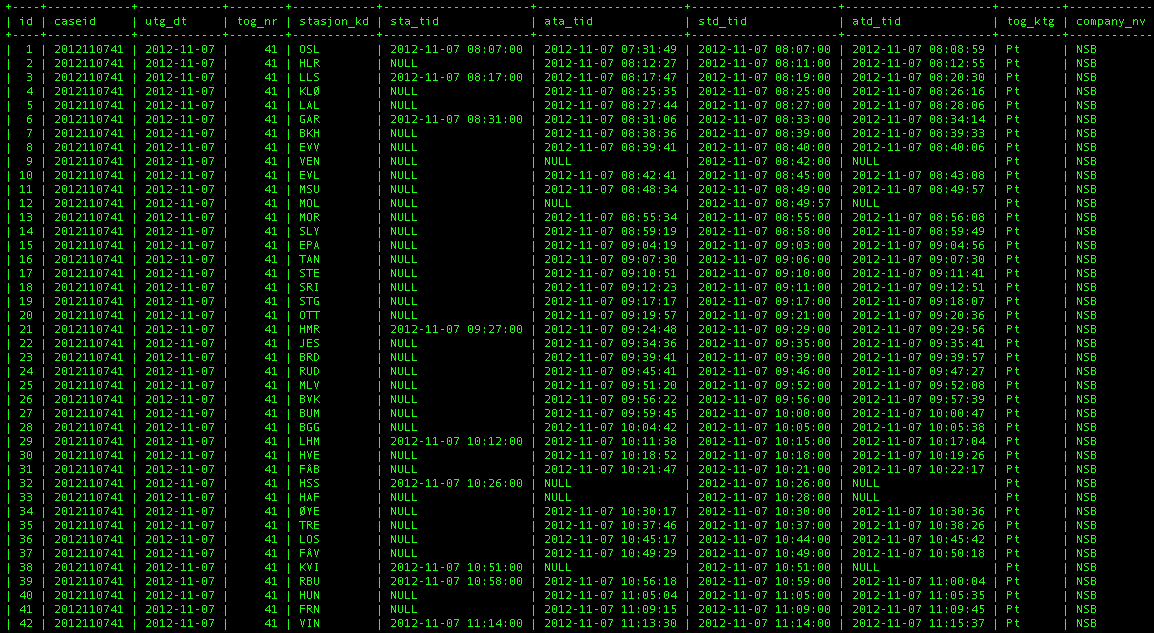
\includegraphics[width=\textwidth,center]{trafikkdata.png}
	\caption[TIOS Punctuality data]{TIOS Punctuality data \cite{sintefPresis}}
	\label{fig:jernbaneverket-trafikkdata}
\end{figure}

Since the set of data stored in TIOS, stores every train that passes every 
measurement point, and the corresponding time point , is is possible
to use the same set to calculate where every crossing between different trains
happens. The usage of the same set is possible since one can compare the time 
stamps of the passing of each station to another train.\\

When the speed restrictions are registered, they are stored in their own set of
data which is based on the users filling out different forms. The speed
restriction sets are based on forms filled out by users, and cover both
scheduled work and unscheduled work. Examples of scheduled work can be
improvement on infrastructure, and example of unscheduled work can be destroyed
tracks due to flooding. \\

Analyzing large different sets of data which might originate from different
sources, will be required when a method shall be aware of the stakeholder.
When developing such a method, one also needs to have a good way of limiting
the visual representation of the data to avoid filling the display with to much
information.
% section data_sets (end)

\section{Aggregation} % (fold)
\label{sec:back_aggregation}

When using the hierarchy of relevant stakeholders presented in \Ref{sec:back_stakeholders}
and the large sets of data mentioned in \Ref{sec:back_data_sets}, a
good way to limit the amount of data presented is to aggregate over the sets of
data based on hierarchy.

If one look at the example hierarchy presented in Section
\Ref{sec:back_stakeholders}, an example of such an aggregation is as
follows. The segment director wants information of every station along the
segment. The Stretch director wants summarized information from each segment, which is
aggregated from the stations. The area director wants information of every
stretch, which is aggregated from each segment.

When one is aware of the different level of details each type of stakeholder
wants, the aggregation quickly becomes a useful way of determining the
necessary data.

% section aggregation (end)

% !TEX root=../../thesis.tex
\section{Examples}
\label{sect:backgroundExamples}
This section will present some relevant examples and try to explain what these
examples tries to present.
\subsection{Zugmonitor}
\label{sub:subsection_zugmonitor}

In the Zugmonitor (see \vref{fig:zugmonitor}) example each long-distance 
trains in the German railway network has been plotted as a arrow on a German 
map. To illustrate the punctuality of each train, a colored circle has been 
added to each arrow if the train is delayed with varying color depending on 
how big the delay is. It has also been implemented a time line functionality 
to see how the trains are on each step of the routes. This time line 
functionality has both a play forward function and manually drag along the 
time line.

\begin{figure}[!htbp]
	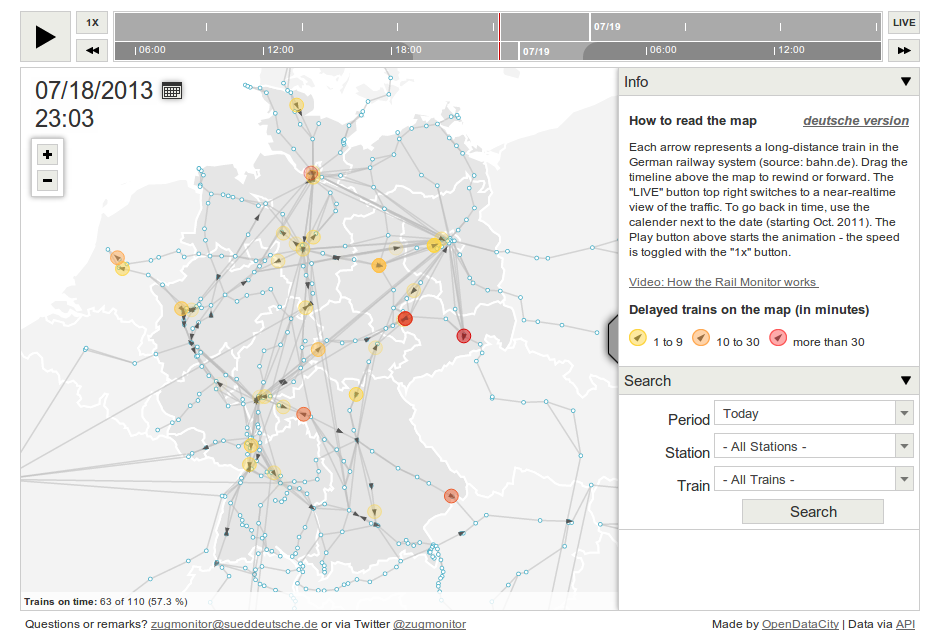
\includegraphics[width=\textwidth,center]{zugmonitor.png}
	\caption[Zugmonitor]{Zugmonitor \cite{zugmonitor}}
	\label{fig:zugmonitor}
\end{figure}
\pagebreak

\clearpage
\subsection{Vaguely live map of trains in the United Kingdom}
\label{sub:subsection_ukLiveMap}

This is a map which plots the relative location of each train in the United
Kingdom (see \vref{fig:ukLiveMap}). The plot fetches the departure time from the 
National Rail website and calculates the relative location. The plot does not
indicate whether or not the trains are on schedule or delayed, this must be
done either manually or for instance checking a time table\cite{trainTimesUK}.
Both the map and time table is developed on hobby basis by the same person. 

\begin{figure}[!htbp]
	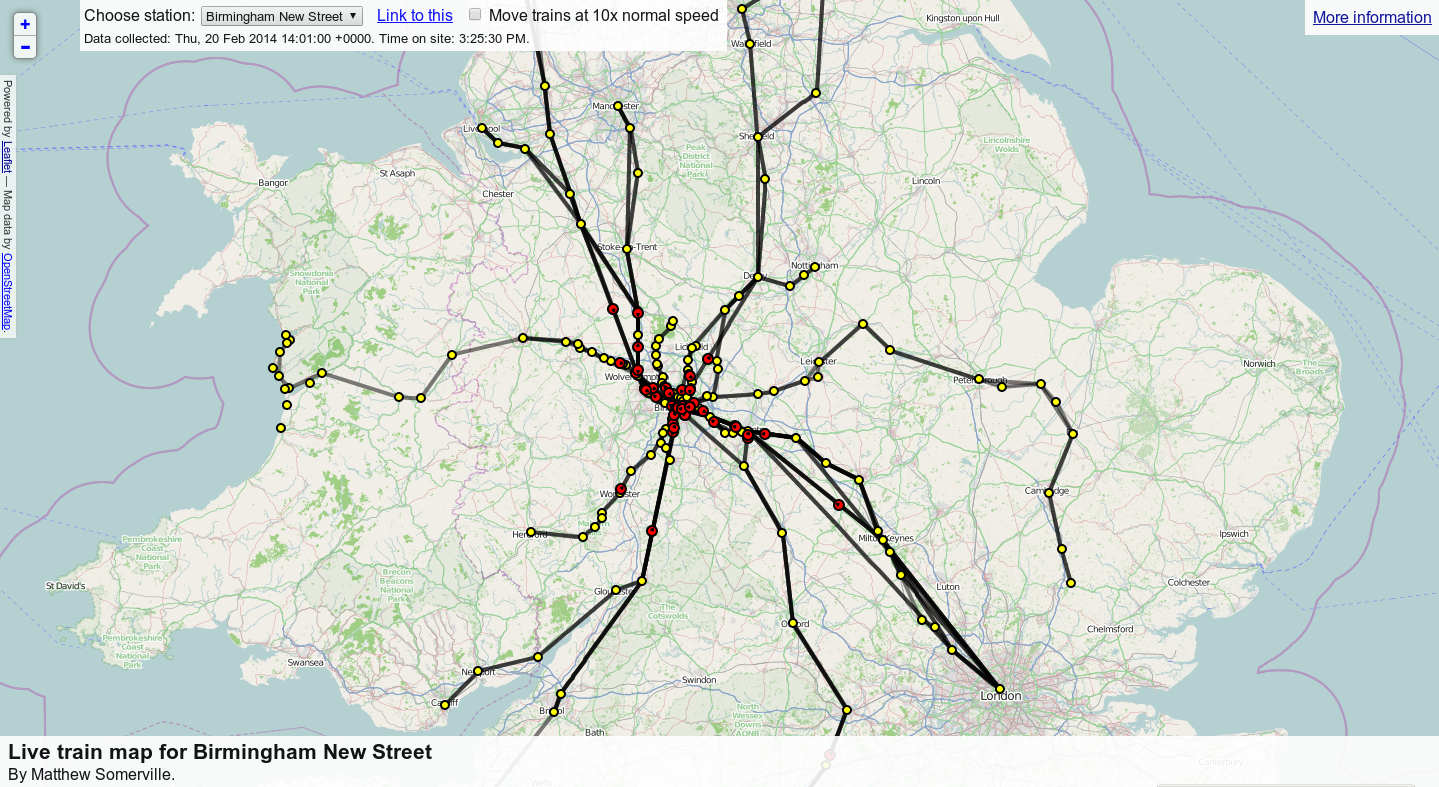
\includegraphics[width=\textwidth,center]{live-train-map-for-Birminingham-new-street.png}
	\caption[UK live map]{UK live map \cite{ukLiveMap}}
	\label{fig:ukLiveMap}
\end{figure}
\pagebreak

\clearpage
\subsection{MUNI Light Rail}
\label{sub:subsection_muniLightRail}

This a train graph based on the N-Judah line on the Muni Metro light railway line in San Francisco (see \vref{fig:muniLightRail}). 
This chart plots the schedule of the each train and the actual time each train 
uses. The chart auto updates each 10 seconds, and combined with being able 
to spot the difference between the schedule and the actual time, makes it easy 
spot the delay of each train. As with \vref{sub:subsection_ukLiveMap} it has been 
developed on a hobby basis.

\begin{figure}[!htbp]
	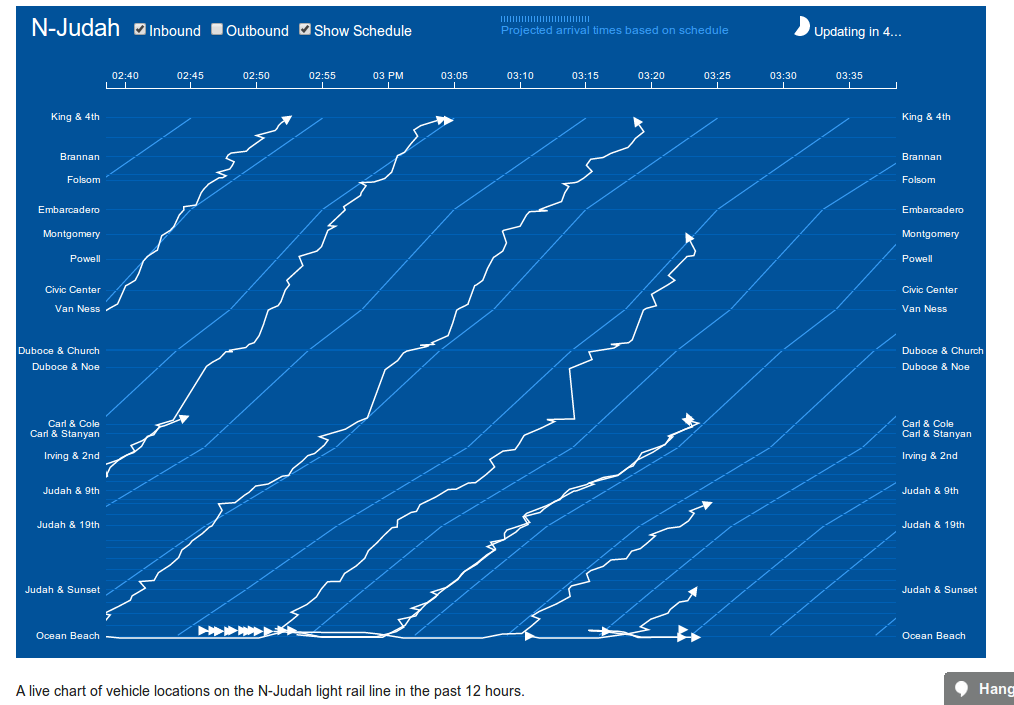
\includegraphics[width=\textwidth,center]{visualizing-transit-delays.png}
	\caption[MUNI Light Rail]{MUNI Light Rail \cite{muniLightRail}}
	\label{fig:muniLightRail}
\end{figure}
\pagebreak


\clearpage
\subsection{MiseryMap}
\label{sub:subsection_zugmonitor}

The MiseryMap (see \vref{fig:miserymap}) shows how much different airports and 
the routes between them are delayed. It also have a playback function to see
how the delays are throughout the day. This plot also shows some weather so it
may be possible to spot if the delays to be blamed on uncontrollable
conditions. 

\begin{figure}[!htbp]
	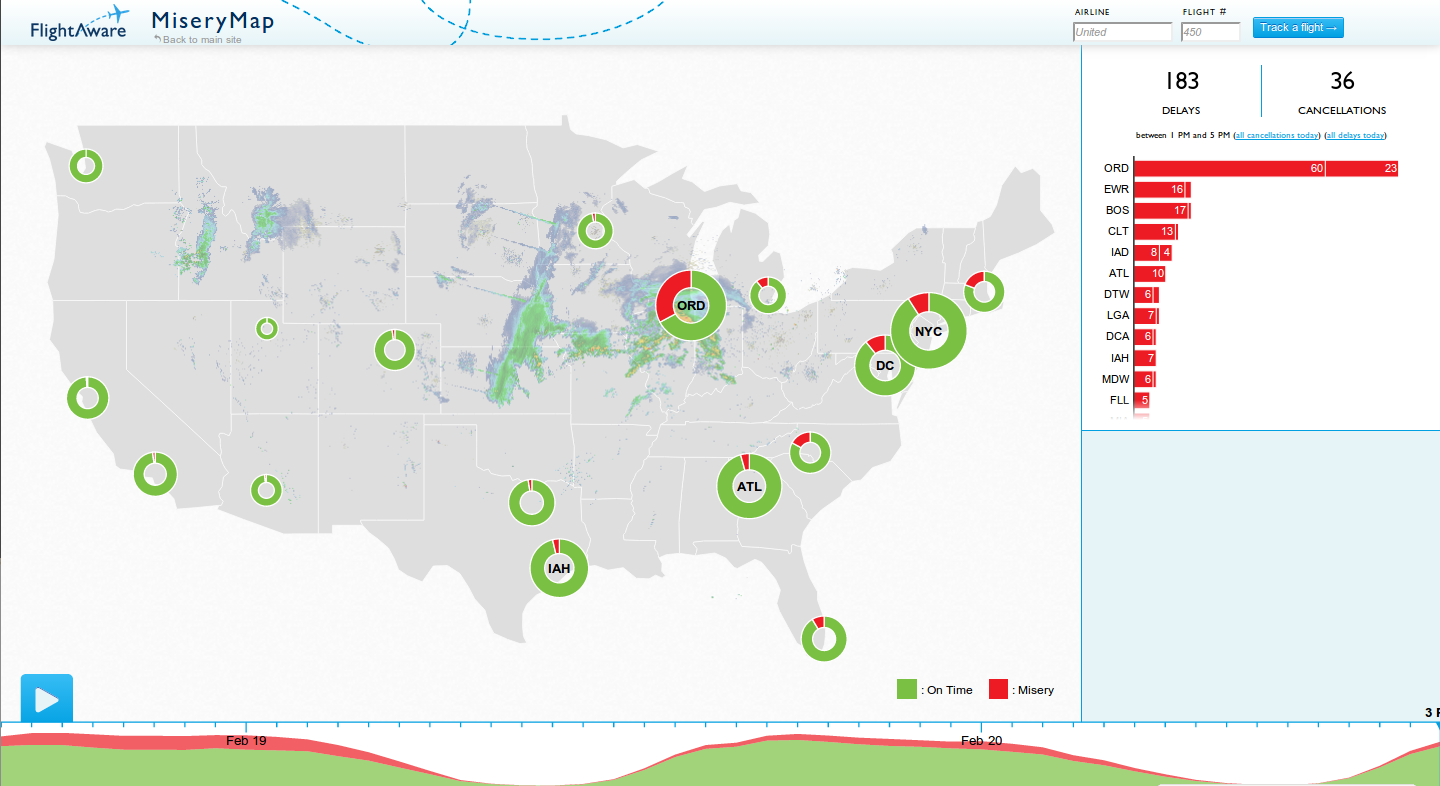
\includegraphics[width=\textwidth,center]{MiseryMap.png}
	\caption[MiseryMap]{MiseryMap \cite{flightAware:MiseryMap}}
	\label{fig:miserymap}
\end{figure}
%\pagebreak
 
\clearpage
\subsection{Norwegian National Rail Administration}
\label{sub:subsection_jernbaneverket}

Jernbaneverket is the Norwegian governments agency for railway services \cite{jernbaneverketAbout}.
This means that they are responsible for all the railway network in Norway.
Because of this, they also collect in data from points that each train passes, see \vref{fig:jernbaneverket-trafikkdata}. 
Based on this, they have recently released a map (see \vref{fig:jernbaneverket-punklighet}) over the punctuality on each stretch. This is a 
interactive map which shows a pop-up box containing the punctuality of the 
stretch clicked on, and this pop-up also shows which routes are using this 
stretch. The map, does not however, show more information if the user zooms 
inn, which is possible within the map itself, and has a static view of Norway 
and the railway. This map only shows the punctuality for passenger trains, and
not freight trains and/or both.\\ 

To analyze each stretch, on a detail level of between each station,
Jernbaneverket has a internal system called TIOS (see \vref{fig:jernbaneverket-tios}).
This is a train graph which plots all trains that passes between all stations,
in this example between Oslo S and Drammen, where the red lines means planned
time, black lines is actual time and the red circle indicates a reason code. 

\begin{figure}[!htbp]
	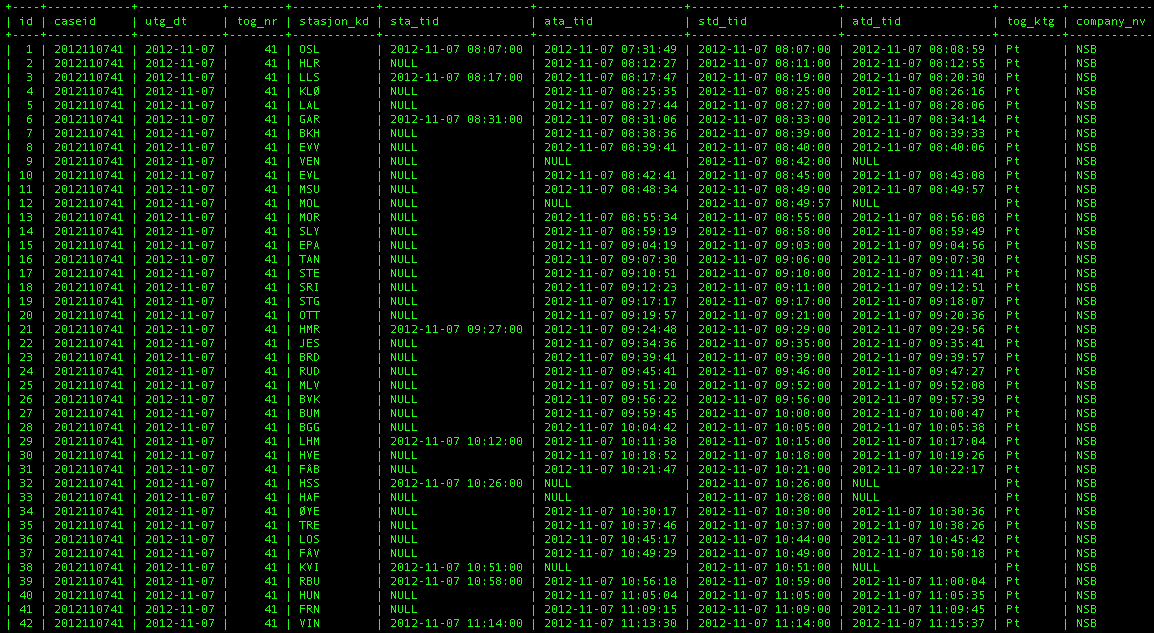
\includegraphics[width=\textwidth,center]{trafikkdata.png}
	\caption[Traffic data]{Traffic data	\cite{sintefPresis}}
	\label{fig:jernbaneverket-trafikkdata}
\end{figure}
\pagebreak

\begin{figure}[!htbp]
	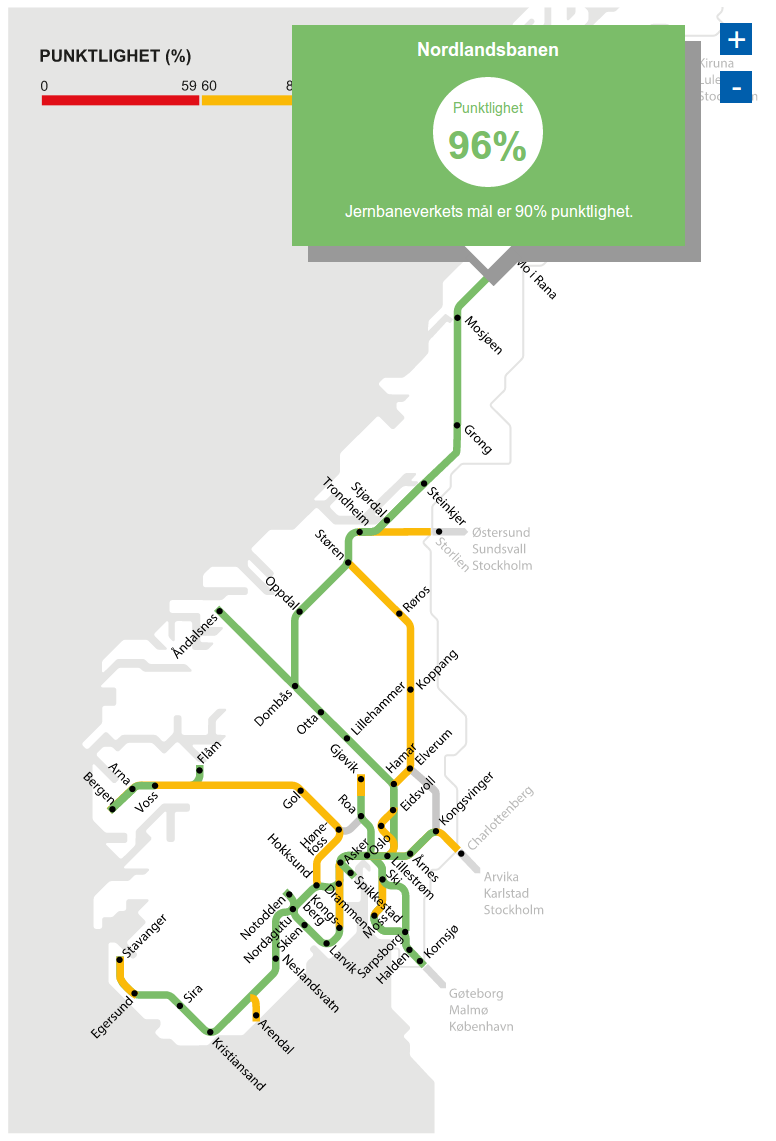
\includegraphics[height=\textheight,center]{jernbaneverket-punklighet.png}
	\caption[JBV Punctuality map]{JBV Punctuality map \cite{jernbaneverketPunklighetKart}}
	\label{fig:jernbaneverket-punklighet}
\end{figure}
\pagebreak

\begin{figure}[!htbp]
	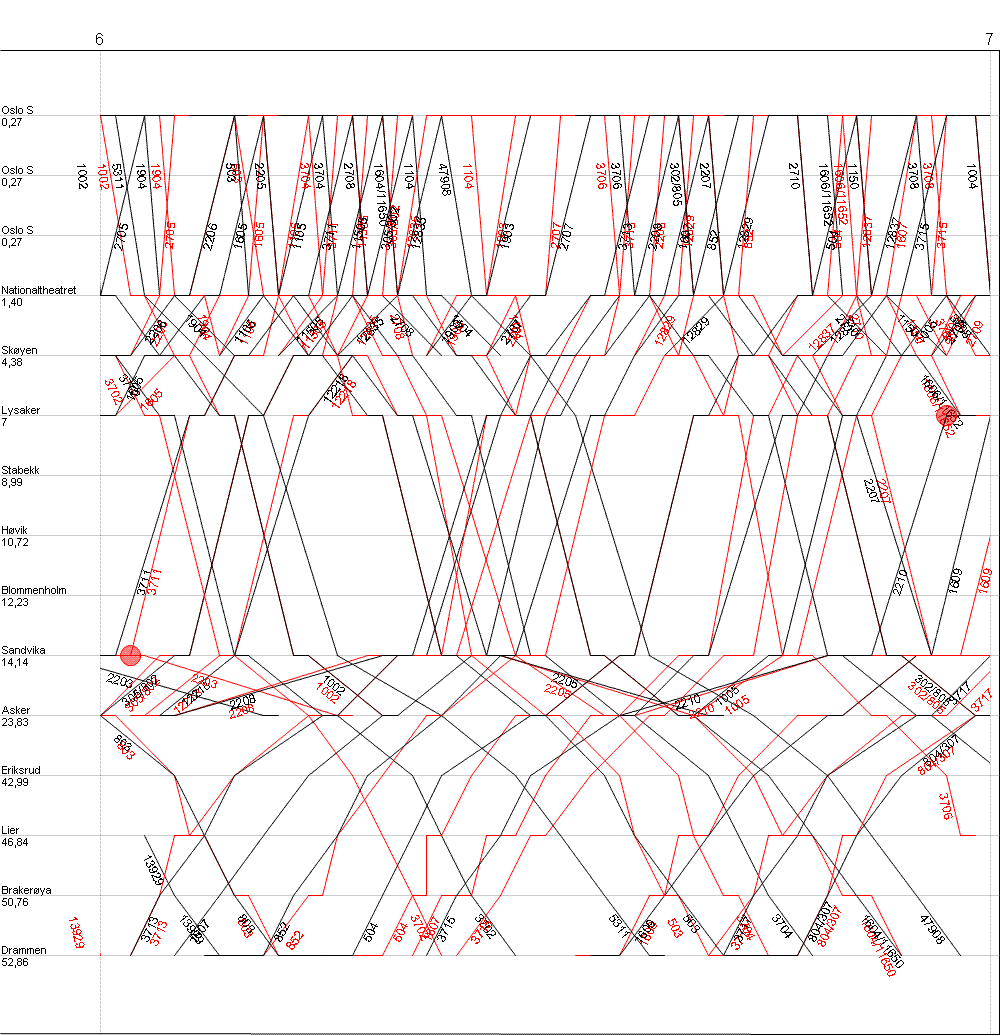
\includegraphics[width=\textwidth,center]{tios.png}
	\caption[TIOS]{TIOS\cite{jernbaneverketPunklighetKart}}
	\label{fig:jernbaneverket-tios}
\end{figure}
\pagebreak


\clearpage
\subsection{Tåg.info}
\label{sub:subsection_taag.info}

Tåg.info\cite{taagInfo} is a Swedish system that tracks SJ\cite{svenskaJernban} trains. The
service gathers and processes data from Trafikverket\cite{trafikverket}. As
with Cargonet (section \vref{sub:subsection_cargonet}), it provides a method (\vref{fig:taag-info-kart}) of
tracking live trains and visually see whether the trains are on schedule or
delayed. 

Tåg.info also provides a method of analyzing national delays by presenting
graphs, \vref{fig:taag-info-historik}. The service presents both a bar-chart
which presents the minutes of delays and the accumulated delays per day, and a
pie chart of the current status.

\begin{figure}[!htbp]
	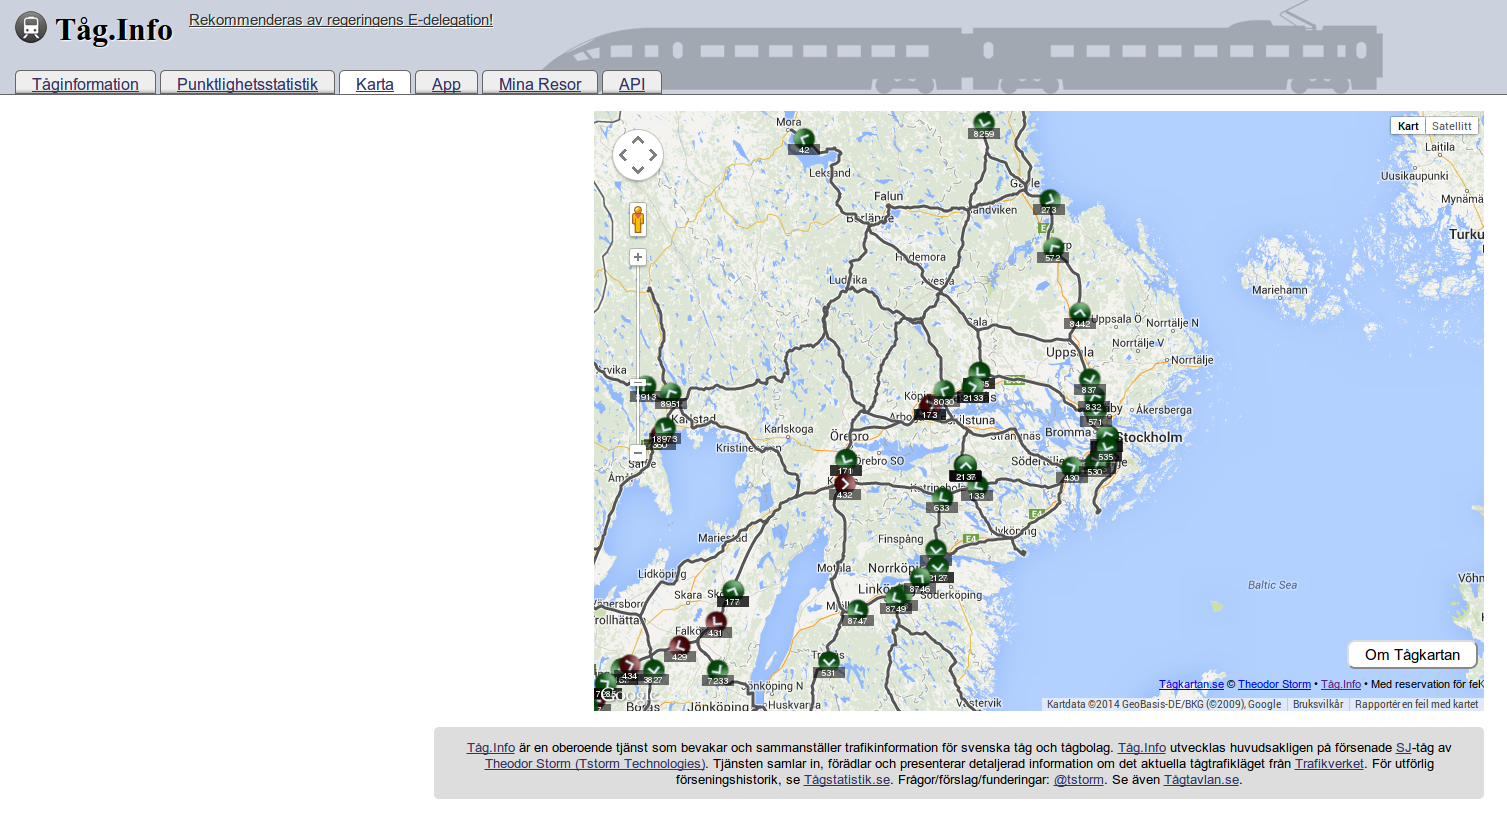
\includegraphics[width=\textwidth,center]{taag-info-kart.png}
	\caption[Tåg.info map]{Tåg.info map
	\cite{taagInfo}}
	\label{fig:taag-info-kart}
\end{figure}
\pagebreak

\begin{figure}[!htbp]
	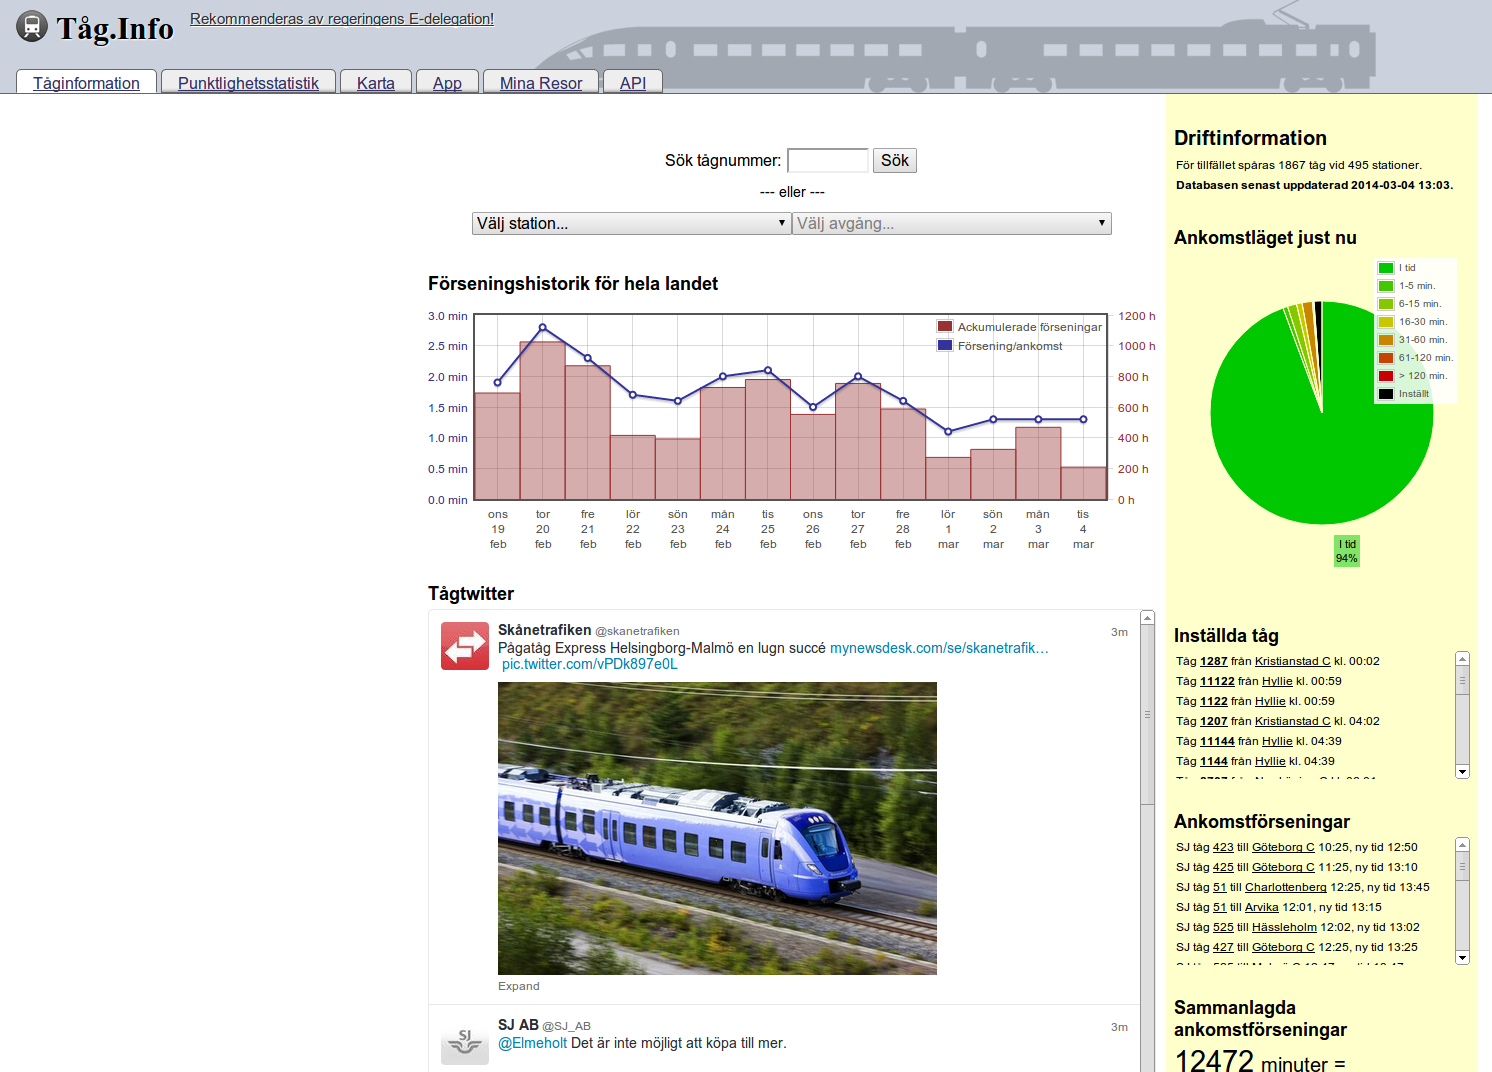
\includegraphics[width=\textwidth,center]{taag-info-historik.png}
	\caption[Tåg.info history]{Tåg.info history
	\cite{taagInfo}}
	\label{fig:taag-info-historik}
\end{figure}
\pagebreak


\clearpage
\subsection{SINTEF Presis}
\label{sub:subsection_sintefPresis}

The PRESIS\cite{sintefPresis} project is a project between SINTEF\cite{sintef},
Transportøkonomisk Institutt\cite{transportOkonomiskInstitutt},
NTNU\cite{ntnu}, Jernbaneverket(section \vref{sub:subsection_jernbaneverket}) and the train operators. It is meant to
systematicly improve the precision level in the railway system by developing
methods, tools, and processes. In this project it has been developed several
prototypes for analyzing train delays. 

A interaction plot, see \vref{fig:krysningsinteraksjon}, plots the interaction
between two selected trains at a selected station. This makes it easy to see 
if one train in delayed, how it might affect another train. Since it only
plots between two trains, it makes it tedious to track large delays back 
throughout all interaction a train may have to find the source of the delay.
This makes it useful for individual trains, but makes it difficult to use if
one might look at the entire railway network or a large portion. \\

Publicly and internally it may differ if a train is delayed or not. Publicly
statistically data only shows delays on the final destination of the train, all
station along the route only shows there and then on information screens.
Since Jernbaneverket collects data from all signal points along the route (see \vref{fig:jernbaneverket-trafikkdata}), they
are able to track and plot the delays the train may experience along the route
and not only at the end station. The PRESIS project has develop a prototype for
such a plot, see \vref{fig:live-punklighet}. Here the circles represent a
station and the lines between the station have different 
colors which represent the punctuality between the stations, and the data which
it's based on are listed to the right. They have also made it possible to get a
time used over distance plot (see \vref{fig:plot-spc-for-strekning}) based on
the selected data in the Punctuality for routes plot. 

A plot based on time over distance, \ref{fig:plot-spc-for-strekning}, plots the
actual time used by all trains that have driven that stretch in the selected
time period along with the running average. This makes it possible where and
when trains have experienced problems on the selected stretch. They also have a
prototype plot which plots time used on station (see \vref{fig:plot-spc-for-stasjonsopphold})
and other prototypes which is similar, just focusing on other parts of the
process.  %Bidragsplot, ikke tatt med.



%\begin{figure}[!htbp]
%	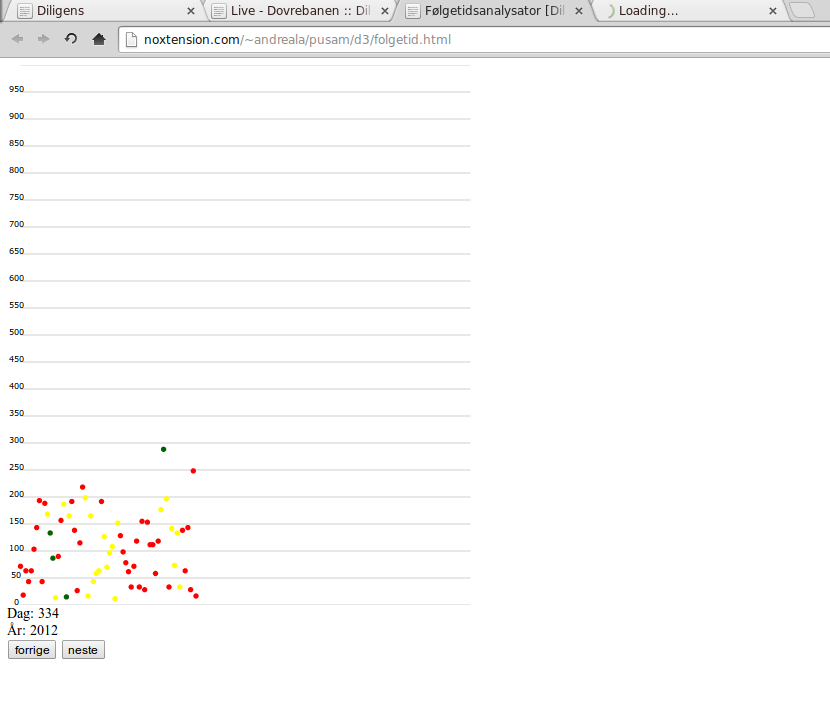
\includegraphics[width=\textwidth,center]{folgetid.png}
%	\caption[folgetid]{folgetid \cite{sintefPresis}}
%	\label{fig:folgetid}
%\end{figure}
%\pagebreak

%\begin{figure}[!htbp]
%	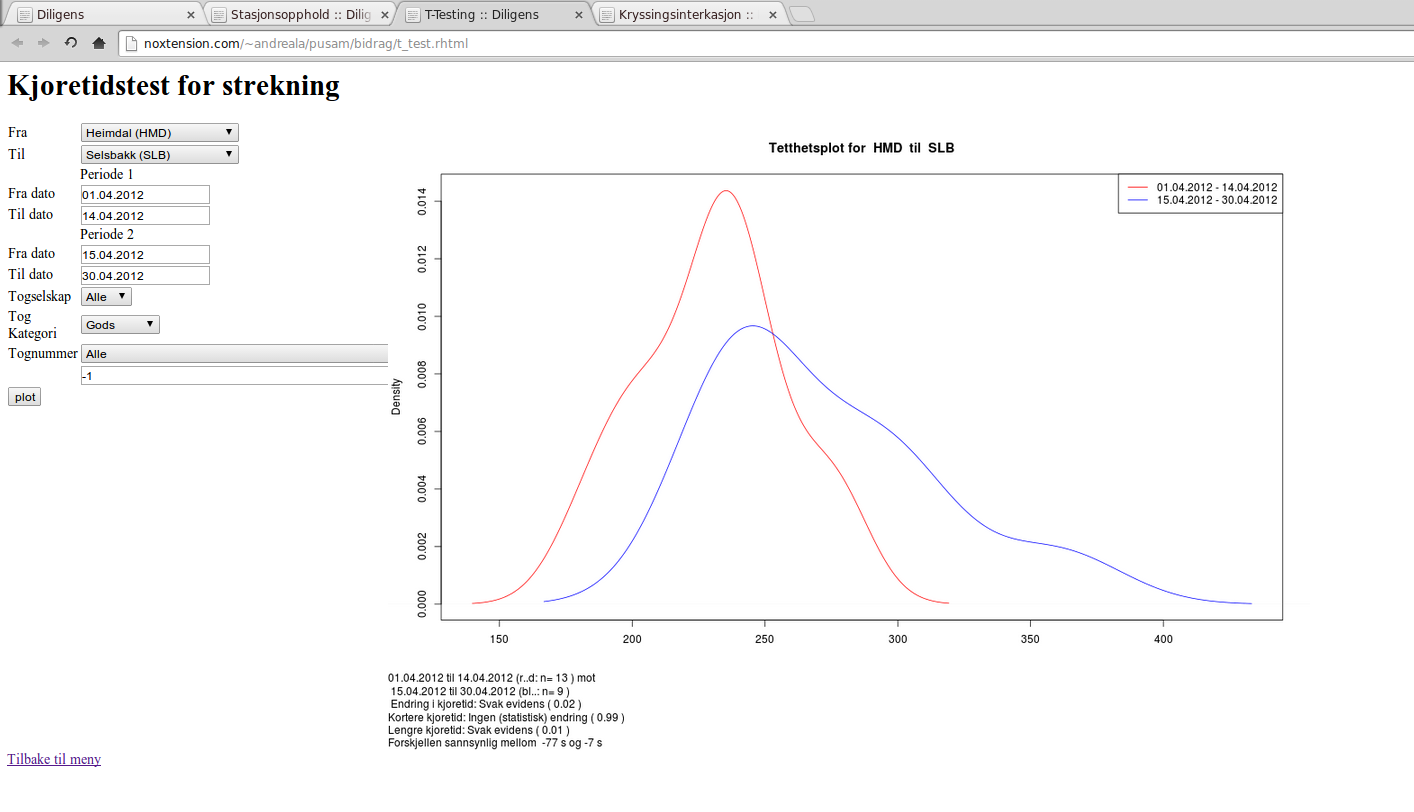
\includegraphics[width=\textwidth,center]{kjoretidstes-strekning.png}
%	\caption[Density plot based on driving time]{Density plot based on driving %time \cite{sintefPresis}}
%	\label{fig:kjoretidstes-strekning}
%\end{figure}
%\pagebreak

\begin{figure}[!htbp]
	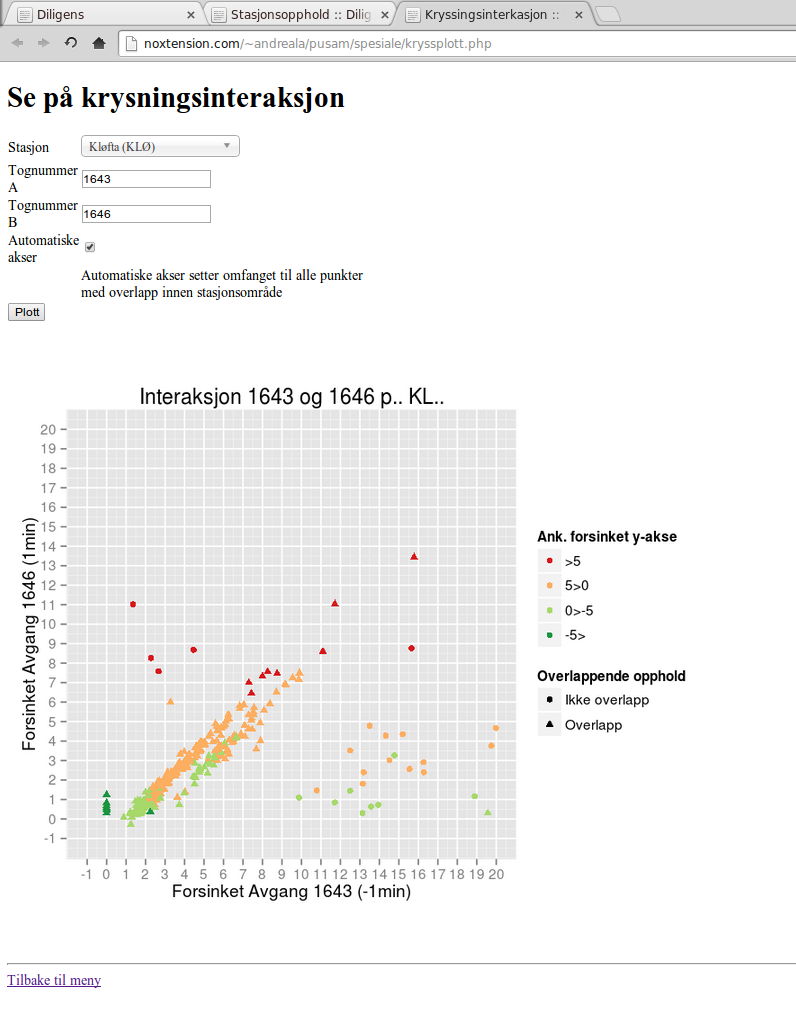
\includegraphics[width=\textwidth,center]{krysningsinteraksjon.png}
	\caption[Train interaction plot]{Train interaction plot \cite{sintefPresis}}
	\label{fig:krysningsinteraksjon}
\end{figure}
\pagebreak

\begin{figure}[!htbp]
	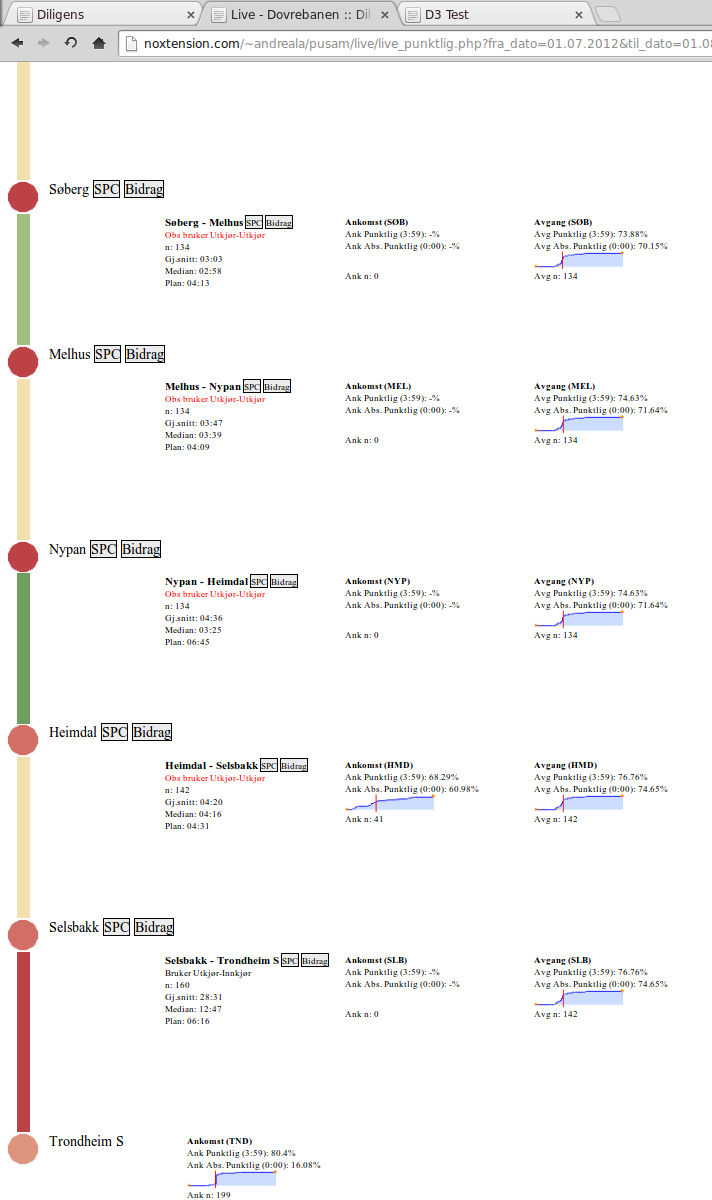
\includegraphics[height=\textheight,center]{live-punklighet.png}
	\caption[Route punctuality]{Route punctuality\cite{sintefPresis}}
	\label{fig:live-punklighet}
\end{figure}
\pagebreak

\begin{figure}[!htbp]
	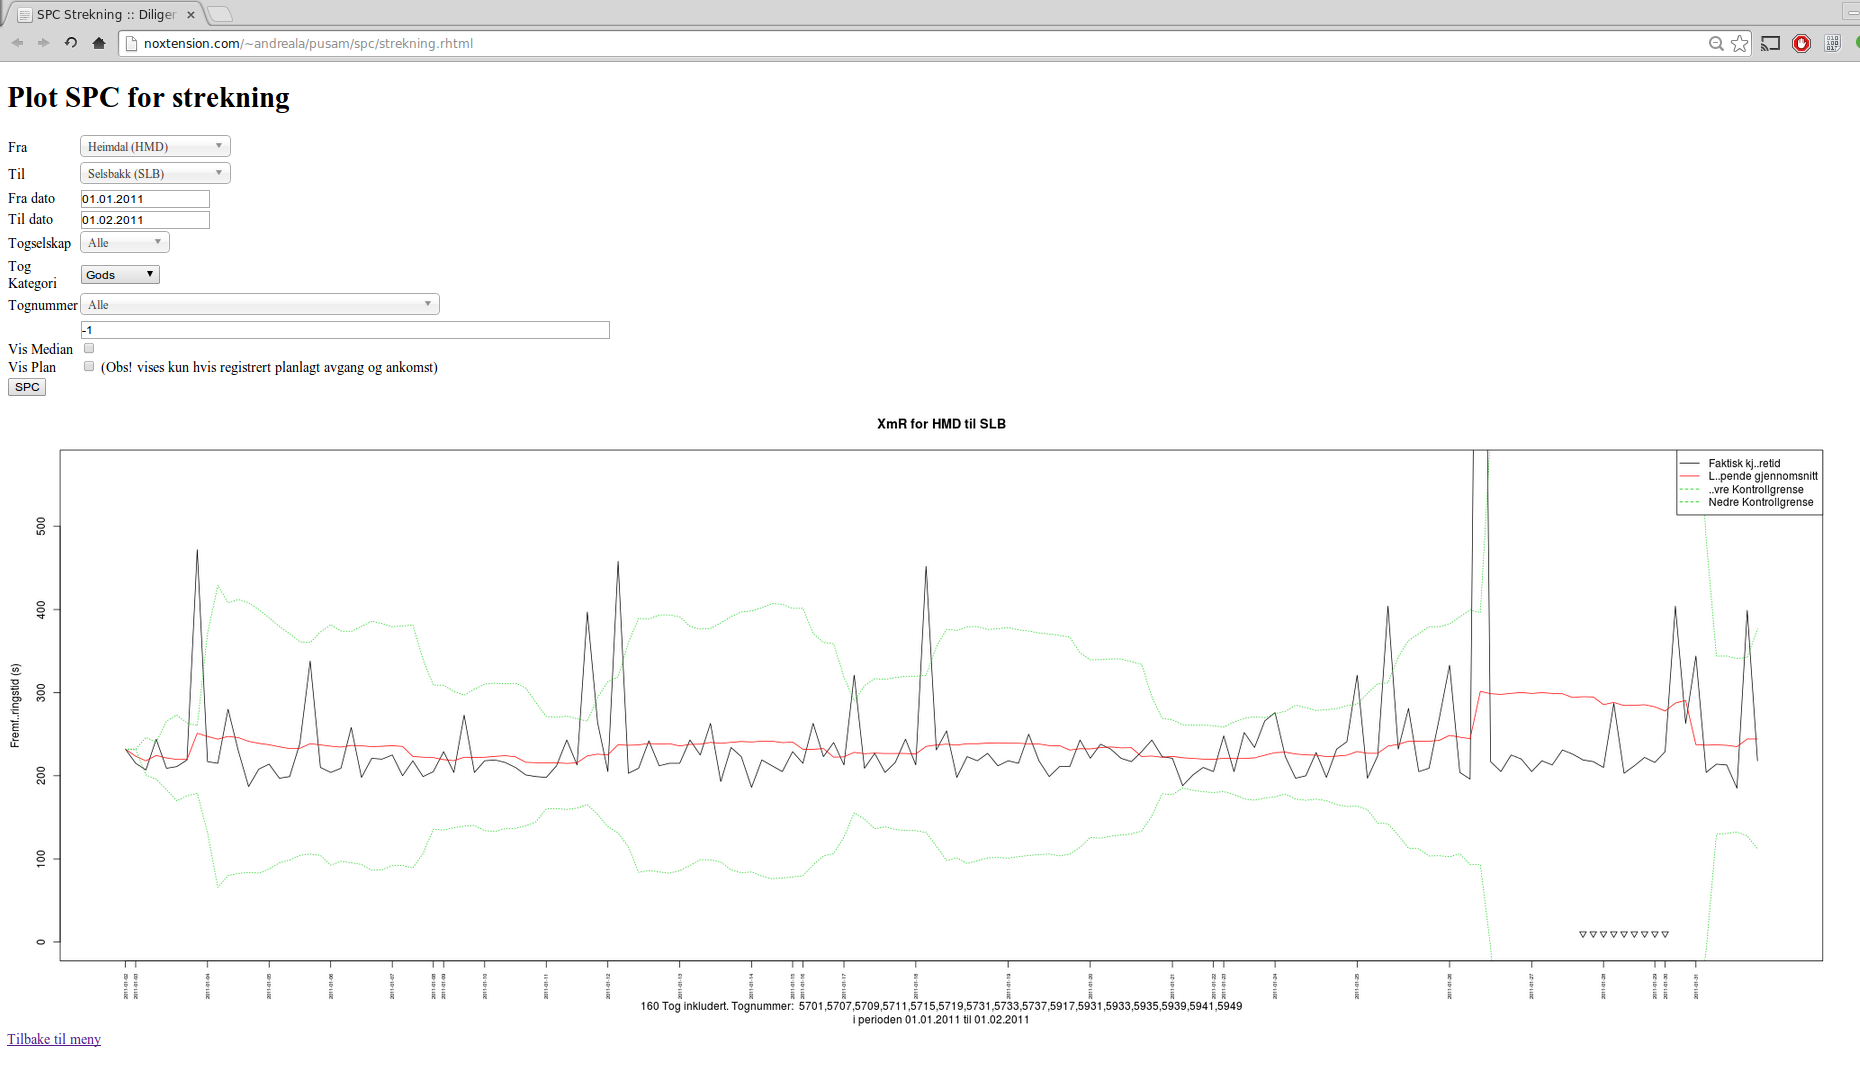
\includegraphics[width=\textwidth,center]{plot-spc-for-strekning.png}
	\caption[SPC Stretch]{SPC Stretch \cite{sintefPresis}}
	\label{fig:plot-spc-for-strekning}
\end{figure}
\pagebreak

\begin{figure}[!htbp]
	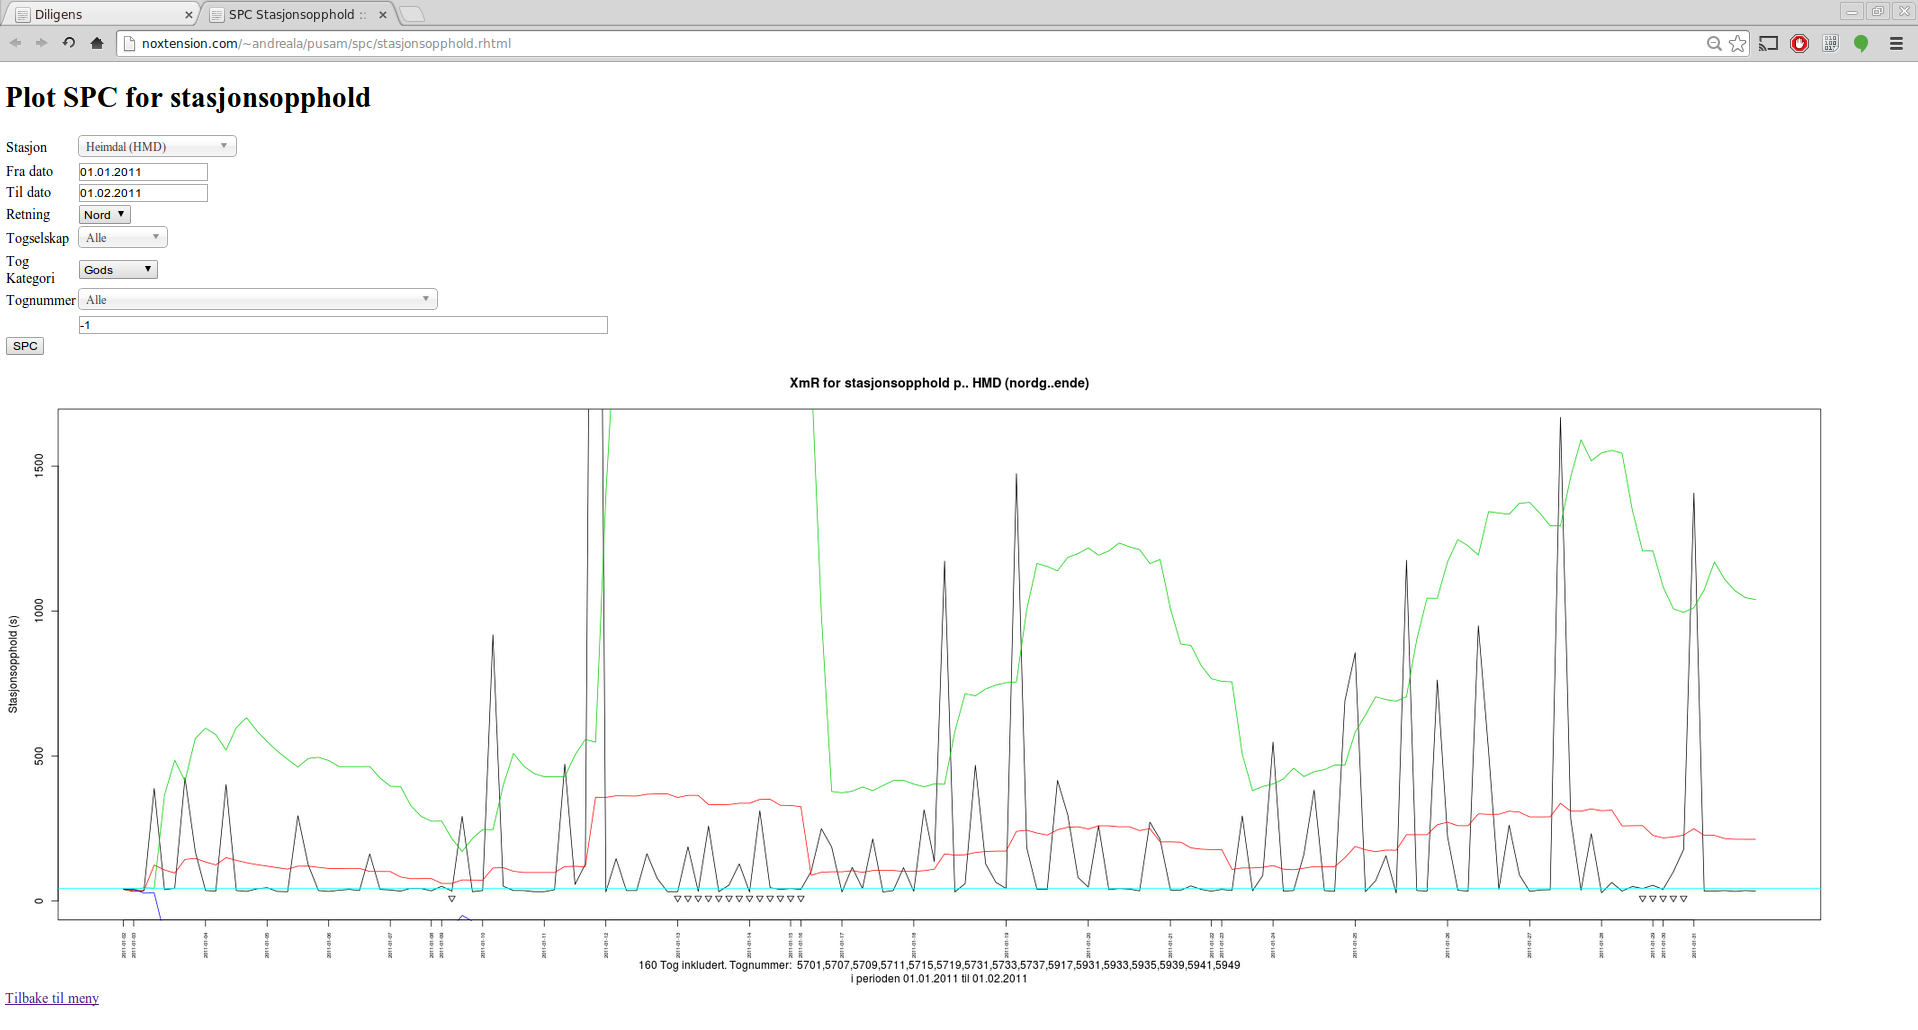
\includegraphics[width=\textwidth,center]{plot-spc-stasjonsopphold.png}
	\caption[SPC Station]{SPC Station \cite{sintefPresis}}
	\label{fig:plot-spc-for-stasjonsopphold}
\end{figure}
\pagebreak

\begin{figure}[!htbp]
	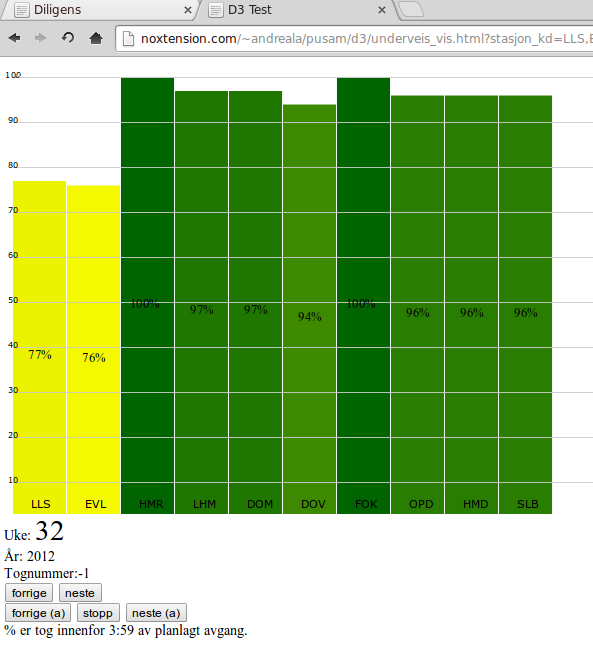
\includegraphics[width=\textwidth,center]{ukespunklighet.png}
	\caption[Weekly punctuality]{Weekly punctuality\cite{sintefPresis}}
	\label{fig:ukespunklighet}
\end{figure}
\pagebreak

\clearpage
\subsection{Cargonet} % (fold)
\label{sub:subsection_cargonet}

% subsection subsection_sintefPresis (end)
Cargonet is a Norwegian which provides intermodal transport on rails. To 
provide a effective tracking service for the customers, Cargonet provides a 
internal service for the users which tracks all trains belonging to Cargonet.
As can be seen on \vref{fig:cargonet}, it only shows a picture of the current
status of each train, it lacks the possibility to analyze both each stretch 
individually  and analyze trains and stretches in time.

\begin{figure}[!htbp]
	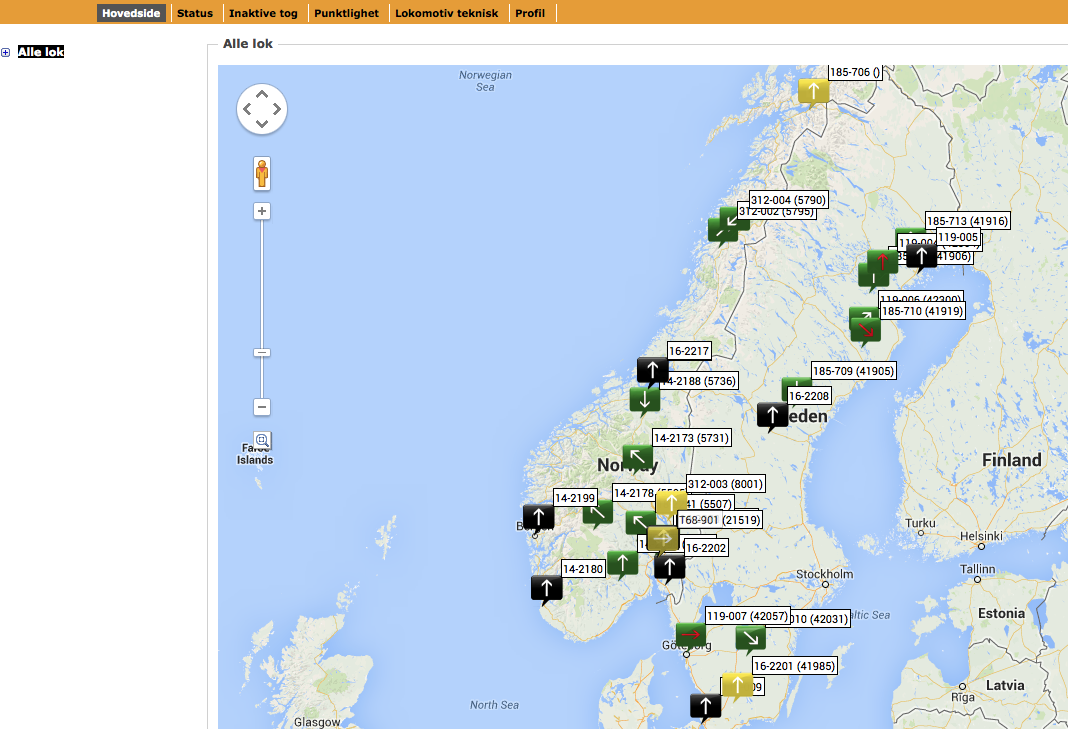
\includegraphics[width=\textwidth,center]{cargonet.png}
	\caption[Cargonet]{Cargonet \cite{cargonet}}
	\label{fig:cargonet}
\end{figure}

\begin{itemize}
	\item [] \textbf{How to read \ref{fig:cargonet}}
	\item Red arrow:\hspace{4ex} Delayed.
	\item White arrow:\hspace{4ex} On time.
	\item Red box:\hspace{4ex} Locomotive driven 2km without carriages.
	\item Black box:\hspace{4ex} Locomotive without carriages.
	\item Yellow box:\hspace{4ex} Locomotive on time without schedule, or known position.
\end{itemize}

\pagebreak
% subsection subsection_cargonet (end)

% !TEX root=../../thesis.tex

\section{Defining frameworks} % (fold)
\label{sec:defining_frameworks}
This section will first define the users in the railway network, and then
define framework(s) based on the need of the users and what the examples
presented in section \vref{sect:backgroundExamples} tries to present.

\subsection{User roles in the Norwegian railway network} % (fold)
\label{sub:user_roles_in_the_norwegian_railway_network}

Combined in all the companies with a certain interest in the Norwegian railway 
network there are several types of users which have different perspective of
the railway. 
\begin{table}[!h]\small
	\begin{tabularx}{\textwidth}{|l|l|X|}
		\hline
		Company & User type & Responsibility \\
		\hline
		Jernbaneverket & Traffic director & Responsibility to facilitate that the railway traffic in Norway is safe and reliable\\
		\hline
		Jernbaneverket & Area director & Responsibility to facilitate that the railway traffic in Norway is safe and reliable\\
		\hline
		Jernbaneverket & Segment director & Responsibility to facilitate that the railway traffic in Norway is safe and reliable\\
		\hline
		NSB & Nation responsible & 1 per line (Dovre, Bergen, etc.)\\
		\hline
		NSB & East responsible & 1 per defined area in the east of Norway (Vestfold county, Oslo - Hamar,
		etc.)\\
		\hline
		None & Average Joe & General user interested in train punctuality\\
		\hline
	\end{tabularx}
\caption{User roles in the Norwegian railway network}
\label{table:user_roles}
\end{table}

Based on the perspective of these users, different information is useful and
not all examples in section \ref{sect:backgroundExamples} may be useful. They
may have just a basic interest whether trains are delayed or not, for instance
traveling with trains on holiday; or have a more detailed need to understand
all train delays in the whole network, for instance to make new schedules. 

% subsection user_roles_in_the_norwegian_railway_network (end)

\clearpage
\subsection{Information presented vs information needed} % (fold)
\label{sub:information_presented_vs_information_needed}

Since each project presented in section \vref{sect:backgroundExamples} is
based different type of user accessing it, they present different amount of
information. Since some the projects presented contains different types of
information presentations and they may cover different needs, the following 
definition will be based on the presented figures. 

\begin{table}[!h]\small
	\begin{tabularx}{\textwidth}{|l|l|X|}
		\hline
		User & Need & Figure \\
		\hline
		Traffic director & Overview/detailed for the nation & Responsibility to facilitate that the railway traffic in Norway is safe and reliable\\
		\hline
		Area director & Overview/detailed for the area & Responsibility to facilitate that the railway traffic in Norway is safe and reliable\\
		\hline
		Segment director & Detailed for each segment & Responsibility to facilitate that the railway traffic in Norway is safe and reliable\\
		\hline
		Nation responsible & Detailed for each line & 1 per line (Dovre, Bergen, etc.)\\
		\hline
		East responsible & Detailed for east & 
						\vref{fig:muniLightRail} \newline
						\vref{fig:jernbaneverket-tios} \newline
						\vref{fig:krysningsinteraksjon} \newline
						\vref{fig:plot-spc-for-strekning} \newline
						\vref{fig:plot-spc-for-stasjonsopphold} \newline
						\vref{fig:ukespunklighet}\\
		\hline
		None & Basic & 	\vref{fig:zugmonitor}\newline
						\vref{fig:ukLiveMap} \newline
						\vref{fig:miserymap} \newline
						\vref{fig:jernbaneverket-punklighet}\\
		\hline
	\end{tabularx}
\caption{Information presented vs information needed}
\label{table:information_presented_vs_information_needed}
\end{table}


% subsection information_plotted_vs_information_needed (end)

% section defining_frameworks (end)

 
